\begin{frame}
    \centering
    \textbf{\Large{Iterative solution algorithms}}
\end{frame}

\begin{frame}
    \frametitle{Integral formulation SCF}
    \centering
    \textbf{Kohn-Sham equations}
    \begin{equation}
	\nonumber
	\bigg[-\frac{1}{2}\nabla^2 + \hat{V}\bigg]\orbital_i(r) = \epsilon_i \orbital_i(r)
    \end{equation}

    \vspace{5mm}

    \textbf{Rewrite using} $\mu_i^2 = -2\epsilon_i$
    \begin{align}
	\nonumber
	\Big[-\nabla^2 + \mu_i^2\Big]\orbital_i(r) =&\ -2\hat{V}\orbital_i(r)\\
	\nonumber
	\orbital_i(r) =&-2\Big[-\nabla^2 + \mu_i^2\Big]^{-1}\hat{V}\orbital_i(r)\\
	\nonumber
	\orbital_i =&-2\hat{G}_i\Big[\hat{V}\orbital_i\Big]
    \end{align}

    \vspace{5mm}

    \textbf{Bound-State Helmholtz operator}
    \begin{equation}
	\nonumber
	\hat{G}_if(r) = \int \frac{e^{-\mu_i |r-r'|}}{4\pi|r-r'|}f(r')dr'
    \end{equation}

    \vspace{5mm}

    \centering
    \tiny
    MH Kalos,
    {\it Phys. Rev.}, 
    \textbf{128(4)},
    1791 (1962)\\
    RJ Harrison, GI Fann, T Yanai, Z Gan and G Beylkin,
    {\it J. Chem. Phys.}, 
    \textbf{121},
    11587 (2004)
\end{frame}

\begin{frame}
    \frametitle{Hydrogen atom}
    \centering
    \textbf{Potential operator}
    \begin{equation}
	\nonumber
	\hat{V} = v_{nuc}(r) = -\sum_I\frac{Z_I}{|r-R_I|}
    \end{equation}

    \vspace{5mm}

    \textbf{Smoothed nuclear potential}
    \begin{align}
	\nonumber
	\frac{1}{r} &\approx \frac{erf(r)}{r} +
	\frac{1}{3\sqrt{\pi}}\big(e^{-r^2}+16e^{-4r^2}\big)
    \end{align}

    \vspace{5mm}

    \textbf{One-electron Schr\"{o}dinger equation}
    \begin{equation}
        \nonumber
        \Big[-\frac{1}{2}\nabla^2 + \hat{V}\Big]\psi(r) = E \psi(r)
    \end{equation}

    \vspace{1mm}

    \begin{equation}
        \nonumber
        \psi = -2\hat{G} \Big[\hat{V} \psi \Big]
    \end{equation}

    \vspace{5mm}

    \centering
    \tiny
    RJ Harrison, GI Fann, T Yanai, Z Gan and G Beylkin,
    {\it J. Chem. Phys.}, 
    \textbf{121},
    11587 (2004)
\end{frame}

\begin{frame}
    \frametitle{One-electron algorithm}
    \centering
    \textbf{Power iteration of the BSH operator}
    \begin{equation}
	\nonumber
	\psi^{n+1} = -2G^n\Big[\hat{V} \psi^n\Big]
    \end{equation}

    \vspace{3mm}

    \textbf{Finding roots of the residual}
    \begin{equation}
	\nonumber
	f(\psi) = -2G^n\big[\hat{V} \psi\big] -\psi
    \end{equation}

    \vspace{3mm}

    \textbf{Newton's method}
    \begin{equation}
	\nonumber
	\psi^{n+1} = \psi^n - \Big[J(\psi^n)\Big]^{-1} f(\psi^n)
    \end{equation}

    \begin{equation}
	\nonumber
	\psi^{n+1} = \psi^n - \Big[J(\psi^n)\Big]^{-1}
	\bigg(-2G^n\Big[\hat{V}\psi^n\Big] - \psi^n\bigg)
    \end{equation}

    \vspace{3mm}

    So the direct power iteration is an "inexact" Newton method\\
    where we approximate the Jacobian $J(\psi^n) \approx -1$.
\end{frame}

\begin{frame}
    \frametitle{One-electron algorithm}
    \begin{columns}
    \begin{column}{.50\textwidth}
    \centering
    \textbf{Initialize BSH operator} $\hat{G}^n$
    \begin{equation}
        \nonumber
        \mu^n = \sqrt{-2E^n}
    \end{equation}
    \end{column}

    \begin{column}{.50\textwidth}
    \centering
    \textbf{Power iteration}
    \begin{equation}
	\nonumber
	\tilde{\psi}^{n+1} = -2\hat{G}^n \Big[ \hat{V} \psi^n \Big]
    \end{equation}
    \end{column}
    \end{columns}

    \vspace{5mm}

    \begin{columns}
    \begin{column}{.50\textwidth}
    \centering
    \textbf{Wavefunction update}
    \begin{equation}
	\nonumber
	\Delta\psi^n = \frac{\tilde{\psi}^{n+1}}{\|\tilde{\psi}^{n+1}\|} - \psi^n
    \end{equation}
    \end{column}

    \begin{column}{.50\textwidth}
    \centering
    \textbf{Energy update}
    \begin{equation}
	\nonumber
	\Delta E^n =
        \frac{\langle\tilde{\psi}^{n+1}|\hat{V}|\Delta\tilde{\psi}^n\rangle}
        {\langle\tilde{\psi}^{n+1}|\tilde{\psi}^{n+1}\rangle}
    \end{equation}
    \end{column}
    \end{columns}

    \vspace{10mm}

    \centering
    \textbf{Update wavefunction and energy}
    \begin{align}
	\nonumber
        \psi^{n+1}  &= \psi^n + \Delta \psi^n\\
	\nonumber
        E^{n+1}     &= E^n + \Delta E^n
    \end{align}
\end{frame}

\begin{frame}
    \frametitle{One-electron algorithm}
    \centering
    \textbf{Using the relation}
    \begin{equation}
        \nonumber
        -2\hat{G}^n = \big(\hat{T} - E^n\big)^{-1}
    \end{equation}

    \vspace{5mm}

    \textbf{Manipulating the energy expression}
    \begin{align}
        \tilde{E}^{n+1}
        \nonumber
        &=	\langle\tilde{\psi}^{n+1}| \hat{T}+\hat{V} | \tilde{\psi}^{n+1}\rangle\\
        \nonumber
        &=	\langle\tilde{\psi}^{n+1}|  \hat{T} - E^n  | \tilde{\psi}^{n+1}\rangle
        +	\langle\tilde{\psi}^{n+1}|  E^n + \hat{V}  | \tilde{\psi}^{n+1}\rangle\\
        \nonumber
        &=	\langle\tilde{\psi}^{n+1}|  \hat{T} - E^n  | 
	        -2\hat{G}^n\big[\hat{V}\psi^n\big]\rangle
        +	\langle\tilde{\psi}^{n+1}| E^n + \hat{V} |\tilde{\psi}^{n+1}\rangle\\
        \nonumber
        &= -\langle\tilde{\psi}^{n+1}| \hat{V} |\psi^{n}\rangle
        +	\langle\tilde{\psi}^{n+1}| E^n + \hat{V} |\tilde{\psi}^{n+1}\rangle\\
        \nonumber
        &= E^{n}\langle\tilde{\psi}^{n+1}|\tilde{\psi}^{n+1}\rangle + 
	    \langle\tilde{\psi}^{n+1}| \hat{V} |\Delta\tilde{\psi}^{n}\rangle
    \end{align}

    \vspace{8mm}

    \centering
    \textbf{Energy without kinetic operator}
    \begin{equation}
        \nonumber
        E^{n+1} = E^{n} + 
        \frac{\langle\tilde{\psi}^{n+1}| \hat{V} |\Delta\tilde{\psi}^{n}\rangle}
        {\langle\tilde{\psi}^{n+1}|\tilde{\psi}^{n+1}\rangle}
    \end{equation}
\end{frame}

\begin{frame}
    \frametitle{Hydrogen atom}
    \only<1>{\includegraphics[viewport = 50 430 300 640, clip, scale=1.2]
       {figures/s1Orb_1.pdf}}
    \only<2>{\includegraphics[viewport = 50 430 300 640, clip, scale=1.2]
       {figures/s1Orb_2.pdf}}
    \only<3>{\includegraphics[viewport = 50 430 300 640, clip, scale=1.2]
       {figures/s1Orb_3.pdf}}
    \only<4>{\includegraphics[viewport = 50 430 300 640, clip, scale=1.2]
       {figures/s1Orb_4.pdf}}
    \only<5>{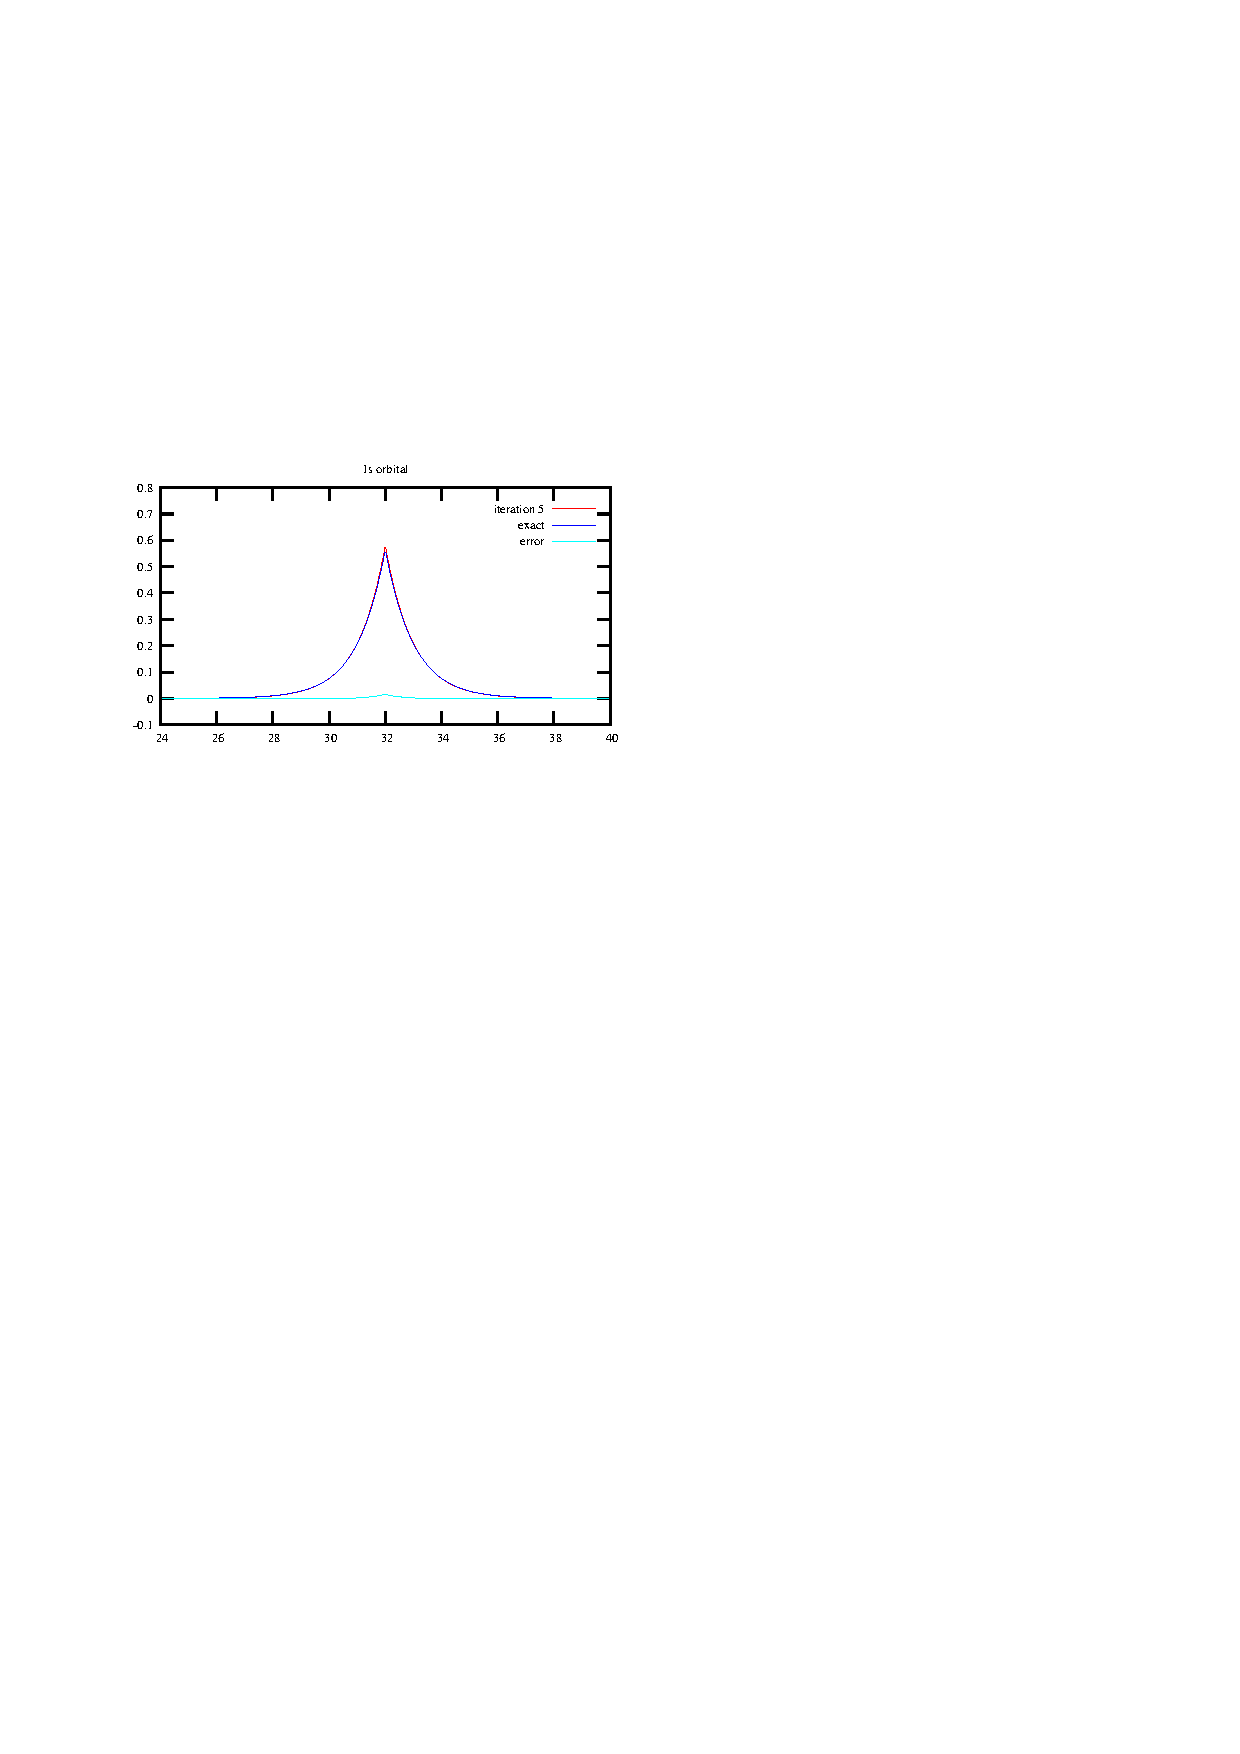
\includegraphics[viewport = 50 430 300 640, clip, scale=1.2]
       {figures/s1Orb_5.pdf}}
    \only<6>{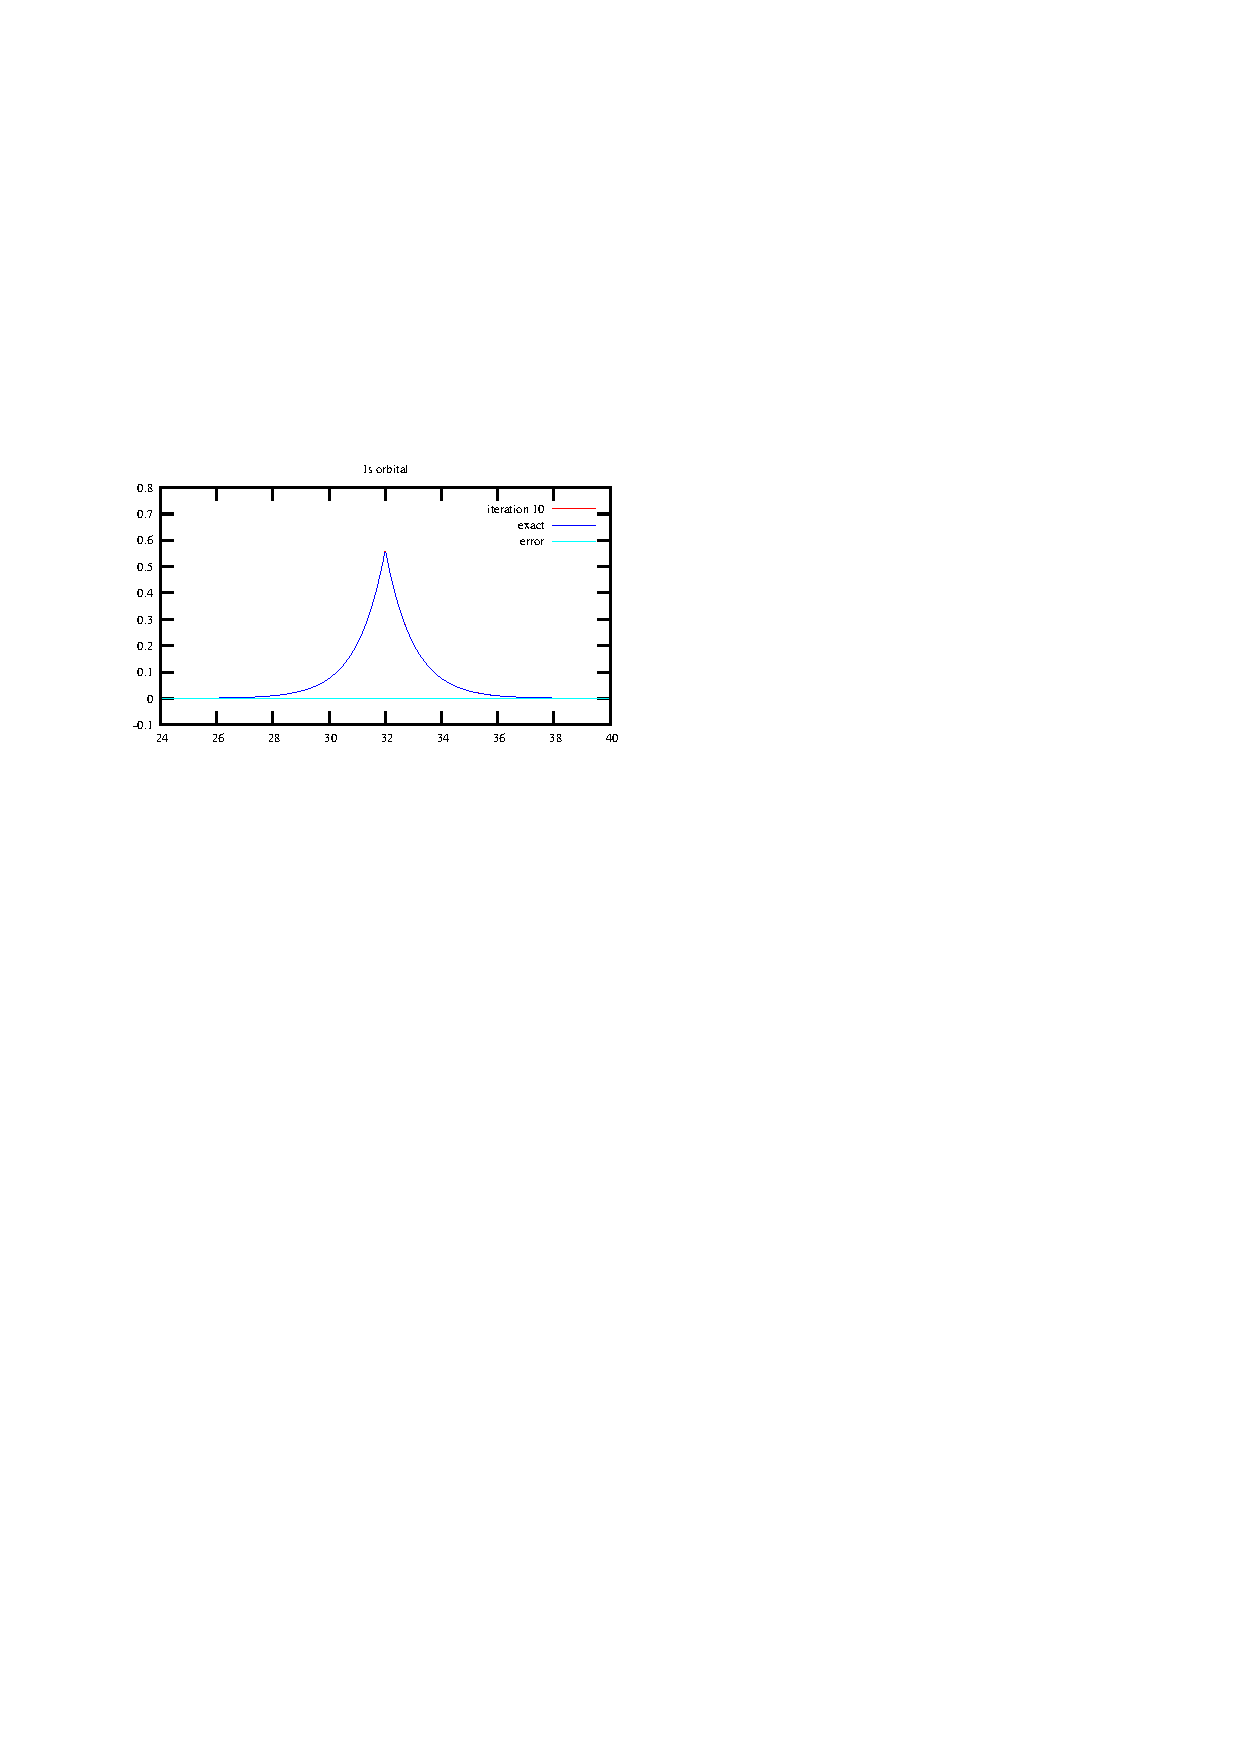
\includegraphics[viewport = 50 430 300 640, clip, scale=1.2]
       {figures/s1Orb_10.pdf}}
\end{frame}

\begin{frame}
    \frametitle{Hydrogen atom}
    \begin{center}
	\includegraphics[scale=1.0, clip, viewport = 50 550 300 730]{figures/h_convergence.pdf}
    \end{center}
\end{frame}


\begin{frame}
    \frametitle{Krylov subspace Accelerated Inexact Newton (KAIN)}
    \begin{columns}
    \begin{column}[b]{0.5\textwidth}
    \centering
    \textbf{Wavefunction history}
    \begin{equation}
	\nonumber
	\psi^0, \psi^1, \dots, \psi^n
    \end{equation}
    \end{column}
    \begin{column}[b]{0.5\textwidth}
    \centering
    \textbf{Residual history}
    \begin{equation}
	\nonumber
	f(\psi^0), f(\psi^1), \dots, f(\psi^n)
    \end{equation}
    \end{column}
    \end{columns}

    \vspace{5mm}

    \centering
    \textbf{Used to find a better approximation to the Jacobian}

    \vspace{10mm}

    The new iterative step is then expanded in the Krylov subspace
    \begin{equation}
	\nonumber
	\delta\psi^n = \sum_i c_i\Big(\psi^i-\psi^n\Big) - 
	\sum_i c_i\Big(f(\psi^i) - f(\psi^n)\Big) - f(\psi^n)
    \end{equation}

    \vspace{5mm}

    by solving the linear system $Ac = b$
    \begin{align}
	\nonumber
	A_{ij} &= \langle\psi^n-\psi^i|f(\psi^n) - f(\psi^j)\rangle\\
	\nonumber
	b_{i}  &= \langle\psi^n-\psi^i|f(\psi^n)\rangle
    \end{align}

    \vspace{5mm}

    \centering
    \tiny
    RJ Harrison,
    {\it J. Comput. Chem.}, 
    \textbf{25(3)},
    328 (2004)
\end{frame}

\begin{frame}
    \frametitle{One-electron algorithm}

    \begin{columns}
    \begin{column}{.50\textwidth}
    \centering
    \textbf{Initialize BSH operator} $\hat{G}^n$
    \begin{equation}
        \nonumber
        \mu^n = \sqrt{-2E^n}
    \end{equation}
    \end{column}

    \begin{column}{.50\textwidth}
    \centering
    \textbf{Power iteration}
    \begin{equation}
	\nonumber
	\tilde{\psi}^{n+1} = -2\hat{G}^n \Big[ \hat{V} \psi^n \Big]
    \end{equation}
    \end{column}
    \end{columns}

    \vspace{5mm}

    \begin{columns}
    \begin{column}{.50\textwidth}
    \centering
    \textbf{Wavefunction update}
    \begin{equation}
	\nonumber
	\Delta\psi^n = \frac{\tilde{\psi}^{n+1}}{\|\tilde{\psi}^{n+1}\|} - \psi^n
    \end{equation}
    \end{column}

    \begin{column}{.50\textwidth}
    \centering
    \textbf{Energy update}
    \begin{equation}
	\nonumber
	\Delta E^n =
        \frac{\langle\tilde{\psi}^{n+1}|\hat{V}|\Delta\tilde{\psi}^n\rangle}
        {\langle\tilde{\psi}^{n+1}|\tilde{\psi}^{n+1}\rangle}
    \end{equation}
    \end{column}
    \end{columns}

    \vspace{5mm}

    \centering
    \textbf{KAIN update}
    \begin{equation}
	\nonumber
        \left(
        \begin{matrix}
        \delta \psi\\
        \delta E
        \end{matrix}
        \right)^{n+1}
        \longleftarrow
        \left(
        \begin{matrix}
        \psi\\
        E
        \end{matrix}
        \right)^n
        ,
        \left(
        \begin{matrix}
        \Delta \psi\\
        \Delta E
        \end{matrix}
        \right)^n
    \end{equation}

    \vspace{5mm}

    \textbf{Update wavefunction and energy}
    \begin{align}
	\nonumber
        \psi^{n+1}  &= \psi^n + \delta \psi^n\\
	\nonumber
        E^{n+1}     &= E^n + \delta E^n
    \end{align}
\end{frame}

\begin{frame}
    \frametitle{Hydrogen atom}
    \begin{center}
	\includegraphics[scale=1.0, clip, viewport = 300 550 560 740]{figures/h_convergence.pdf}
    \end{center}
\end{frame}

\begin{frame}
    \frametitle{Many-electron systems}
    \centering
    \textbf{Potential operator} $0 \leq \alpha \leq 1$
    \begin{equation}
        \nonumber
        \hat{V} = v_{nuc}(r) + v_{el}(r) + v_{xc}(r) - \alpha\hat{K}
    \end{equation}

    \vspace{10mm}

    \begin{columns}
    \begin{column}[b]{0.5\textwidth}
    \centering
    \textbf{Classical nuclear}
    \begin{equation}
        \nonumber
	v_{nuc}(r) = -\sum_I\frac{Z_I}{|r-R_I|}
    \end{equation}
    \end{column}

    \begin{column}[b]{0.5\textwidth}
    \centering
    \textbf{Classical Coulomb}
    \begin{equation}
        \nonumber
        v_{el}(r) = \int \frac{\rho(r')}{4\pi|r-r'|} \ud r'
    \end{equation}
    \end{column}
    \end{columns}

    \vspace{5mm}

    \begin{columns}
    \begin{column}[b]{0.5\textwidth}
    \centering
    \textbf{Exchange-Correlation}
    \begin{equation}
        \nonumber
        v_{xc}(r)
        %= \frac{\delta E_{xc}}{\delta \rho}
        = \frac{\partial F_{xc}}{\partial \rho} - \nabla \cdot \frac{\partial F_{xc}}{\partial \nabla\rho}
    \end{equation}
    \end{column}

    \begin{column}[b]{0.5\textwidth}
    \centering
    \textbf{Hartree-Fock exchange}
    \begin{equation}
        \nonumber
        \hat{K}\phi_p(r) = \sum_i \phi_i(r) \int \frac{\phi_i^\dagger(r')\phi_p(r')}{4\pi|r-r'|} \ud r'
    \end{equation}
    \end{column}
    \end{columns}
\end{frame}

\begin{frame}
    \frametitle{Orthonormalization}
    \centering
    \textbf{Straightforward iteration of the Kohn-Sham equations}
    \begin{equation}
        \nonumber
        \tilde{\phi}_i^{n+1} = -2\hat{G}_i^n \bigg[\hat{V}^n\phi_i^n\bigg]
    \end{equation}
    \textbf{brings all orbitals to the lowest energy eigenfunction}
    
    \vspace{15mm}

    \textbf{Orthonormality must be imposed}
    \begin{equation}
        \nonumber
        \tilde{S}_{ij} = \langle\tilde{\phi}_i|\tilde{\phi}_j\rangle = \delta_{ij}
    \end{equation}

    \vspace{5mm}

    \begin{columns}
    \begin{column}[b]{0.5\linewidth}
    \centering
    \textbf{Gram-Schmidt}
    \begin{equation}
	\nonumber
	\phi_i = \Big(1 - \sum_{j<i}|\phi_j\rangle\langle\phi_j|\Big)\tilde{\phi}_i
    \end{equation}
    \end{column}

    \begin{column}[b]{0.5\linewidth}
    \centering
    \textbf{L\"{o}wdin orthonormalization}
    \begin{equation}
	\nonumber
	\phi_i = \sum_j \tilde{S}_{ij}^{-1/2}\tilde{\phi}_j
    \end{equation}
    \end{column}
    \end{columns}
\end{frame}

\begin{frame}
    \frametitle{Non-canonical orbitals}
    \centering
    \textbf{The non-canonical Kohn-Sham equations}
    \begin{equation}
        \nonumber
        \hat{F}|\phi_i\rangle 
        = \bigg[\sum_j|\phi_j\rangle\langle\phi_j|\bigg]\hat{F}|\phi_i\rangle
        = \sum_jF_{ji}|\phi_j\rangle
    \end{equation}

    \vspace{5mm}

    \textbf{Rewrite using} $\mu_i^2 = -2\lambda_i$
    \begin{align}
        \nonumber
        \bigg[-\frac{1}{2}\nabla^2 + \hat{V}\bigg]\phi_i
        &= \sum_jF_{ji}\phi_j\\
        \nonumber
        \bigg[-\nabla^2 + \mu_i^2\bigg]\phi_i 
        &= -2\bigg[\hat{V}\phi_i - \sum_j\big(F_{ji} -
        \lambda_i\delta_{ji}\big)\phi_j\bigg]\\
        \nonumber
        \phi_i
        &= -2\hat{G}_i\bigg[\hat{V}\phi_i - \sum_j\big(F_{ji} -
        \Lambda_{ji}\big)\phi_j\bigg]
    \end{align}

    \vspace{5mm}

    \begin{columns}
    \begin{column}[b]{0.48\linewidth}
    \centering
    \textbf{Fock matrix}
    \begin{equation}
        \nonumber
        F_{ij} = \langle\phi_i|\hat{T} + \hat{V}|\phi_j\rangle
    \end{equation}
    \end{column}

    \begin{column}[b]{0.48\linewidth}
    \centering
    \textbf{Kinetic matrix}
    \begin{equation}
        \nonumber
        T_{ij}
        = \langle\phi_i|\hat{T}|\phi_j\rangle
        = \frac{1}{2}\langle\nabla\phi_i|\nabla\phi_j\rangle
    \end{equation}
    \end{column}
    \end{columns}
\end{frame}

\begin{frame}
    \frametitle{Localized orbitals}
    \centering
    Total energy invariant under unitary transformations among occupied orbitals
    \begin{equation}
	\nonumber
	\phi_i = \sum_j L_{ij} \phi_i, \qquad \qquad L^\ast L = LL^\ast = I
    \end{equation}

    \begin{columns}
    \begin{column}[b]{0.48\linewidth}
    \centering
    \includegraphics[scale=0.25, clip, viewport = 80 560 600 700]{figures/alkane.pdf}\\
    \includegraphics[scale=0.25, clip, viewport = 80 560 600 700]{figures/can_orb_1.pdf}\\
    \includegraphics[scale=0.25, clip, viewport = 80 560 600 700]{figures/can_orb_2.pdf}\\

    \vspace{2mm}

    \begin{equation}
        \nonumber
        \phi_i =\ -2\hat{G}_i\Bigg[\hat{V}\phi_i
        - (\epsilon_i - \lambda_i)\phi_i\Bigg]
    \end{equation}
    \end{column}

    \begin{column}[b]{0.48\linewidth}
\only<2>{
    \centering
    \includegraphics[scale=0.25, clip, viewport = 80 560 600 700]{figures/loc_orb_1.pdf}\\
    \includegraphics[scale=0.25, clip, viewport = 80 560 600 700]{figures/loc_orb_2.pdf}\\
    \includegraphics[scale=0.25, clip, viewport = 80 560 600 700]{figures/loc_orb_3.pdf}\\

    \vspace{2mm}

    \begin{equation}
        \nonumber
        \phi_i =\ -2\hat{G}_i\Bigg[\hat{V}\phi_i
        - \sum_j(F_{ji} - \Lambda_{ji})\phi_j\Bigg]
    \end{equation}
}
    \end{column}
    \end{columns}

    \vspace{6mm}

    \centering
    \tiny
    S.F. Boys,
    {\it Rev. Mod. Phys.}, 
    \textbf{32:296}
    (1960)\\
    J.M. Foster, S.F. Boys,
    {\it Rev. Mod. Phys.}, 
    \textbf{32:300}
    (1960)
\end{frame}

\begin{frame}
    \frametitle{Many-electron algorithm I}
    \centering
    \textbf{Setup Fock operator} $\hat{F}^n$

    \vspace{5mm}

    \textbf{Compute Fock matrix} $F_{ij}^n = \langle\phi_i^n|\hat{F}^n|\phi_j^n\rangle$

    \vspace{5mm}

    \textbf{Diagonalize/Localize}

    \vspace{5mm}

    \textbf{Iterate BSH operators with} $\lambda_i^n \approx F_{ii}^n$
    \begin{equation}
	\nonumber
        \tilde{\phi}_i^{n+1} = -2\hat{G}_i^n \bigg[\hat{V}^n\phi_i^n -
        \sum_j\big(F_{ji}^n - \Lambda_{ji}^n\big)\phi_j^n\bigg]
    \end{equation}

    \vspace{2mm}

    \textbf{Orthonormalize} $S^{-1/2}$

    \vspace{5mm}

    \textbf{Compute KAIN update} $\delta\phi_i^n$

    \vspace{5mm}

    \textbf{Orthonormalize} $S^{-1/2}$

\end{frame}

\begin{frame}
    \frametitle{Many-electron algorithm I}
    \centering
    \textbf{Overall accuracy kept at} $\epsilon = 10^{-6}$
    \begin{center}
	\includegraphics[scale=1.0, clip, viewport = 50 550 300 740]{figures/accuracy.pdf}
    \end{center}
\end{frame}

\begin{frame}
    \frametitle{Many-electron algorithm I}
    \begin{columns}
    \begin{column}[b]{0.70\linewidth}
        \centering
        \includegraphics[scale=0.8, clip, viewport = 50 550 300 730]{figures/benzene_convergence.pdf}
    \end{column}
    \begin{column}[b]{0.30\linewidth}
        \centering
        \textbf{Benzene}
        \includegraphics[scale=0.1, clip, viewport = 0 0 1000 1200]{figures/benzene.png}

        \vspace{5mm}

    \end{column}
    \end{columns}
\end{frame}

\begin{frame}
    \frametitle{Fock matrix update}
    \centering
    \textbf{Using the relation}
    \begin{equation}
        \nonumber
        -2\hat{G}_i^n = \big(\hat{T} - \lambda_i^n\big)^{-1}
    \end{equation}

    \vspace{3mm}

    \textbf{Manipulating the Fock matrix expression}
    \begin{align}
        \nonumber
        \tilde{F}_{ij}^{n+1}    &= 
        \langle\tilde{\phi}_i^{n+1} |
        \hat{T} + \hat{V}^{n+1}     |
        \tilde{\phi}_j^{n+1}\rangle\\
        \nonumber
			    &= 
        \langle\tilde{\phi}_i^{n+1} |
        \hat{T} - \lambda_j^n       |
        \tilde{\phi}_j^{n+1}\rangle +
        \langle\tilde{\phi}_i^{n+1} |
        \hat{V}^{n+1} + \lambda_j^n |
        \tilde{\phi}_j^{n+1}\rangle\\
        \nonumber
        &\ \ \vdots
    \end{align}

    \textbf{Potential updates}
    \begin{equation}
        \nonumber
        \big(\Delta\tilde{F}_{pot}^n\big)_{ij} =
        \langle\tilde{\phi}_i^{n+1} |
        \hat{V}^n                       |
        \Delta\tilde{\phi}_j^n\rangle + 
        \langle\tilde{\phi}_i^{n+1} |
        \Delta\hat{V}^n                 |
        \phi_j^n\rangle
    \end{equation}

    \vspace{3mm}

    \textbf{Overlap updates}
    \begin{equation}
    \nonumber
        \big(\Delta\tilde{S}_1^n\big)_{ij} =
        \langle\Delta\tilde{\phi}_i^n | \phi_j^n\rangle \qquad \qquad
        \big(\Delta \tilde{S}_2^n\big)_{ij} =
        \langle\tilde{\phi}_i^{n+1} | \Delta\tilde{\phi}_j^n\rangle
    \end{equation}

    \vspace{3mm}

    \centering
    \textbf{Fock matrix without kinetic operator}
    \begin{equation}
        \nonumber
        \tilde{F}^{n+1} = F^{n} + 
        \Delta \tilde{S}_1^n F^n +
        \Delta \tilde{S}_2^n \Lambda^n +
        \Delta \tilde{F}_{pot}^n
    \end{equation}
\end{frame}

\begin{frame}
    \frametitle{Many-electron algorithm II}
    \centering
    \textbf{Setup Fock operator} $\hat{F}^n$

    \vspace{8mm}

    \textbf{Iterate BSH operators with} $\lambda_i^n \approx F_{ii}^n$
    \begin{equation}
	\nonumber
        \tilde{\phi}_i^{n+1} = -2\hat{G}_i^n \bigg[\hat{V}^n\phi_i^n -
        \sum_j\big(F_{ji}^n - \Lambda_{ji}^n\big)\phi_j^n\bigg]
    \end{equation}

    \vspace{2mm}

    \textbf{Compute potential updates} $\Delta\hat{V}^n$

    \vspace{8mm}

    \textbf{Update Fock matrix}
    \begin{equation}
        \nonumber
        \tilde{F}^{n+1} = F^{n} + 
        \Delta \tilde{S}_1^n F^n +
        \Delta \tilde{S}_2^n \Lambda^n +
        \Delta \tilde{F}_{pot}^n
    \end{equation}

    \vspace{5mm}

    \textbf{Orthonormalize} $\tilde{S}^{-1/2}$

    \vspace{5mm}

    \textbf{Diagonalize/localize}

\end{frame}

\begin{frame}
\frametitle{Ground state energy}
\centering
\begin{table}
    \centering
    \begin{tabular}{lr@{.}lr@{.}l}
    \multicolumn{5}{c}{\textbf{LDA energy of Argon (a.u.)}}\\
    \hline
    \hline
                        &\multicolumn{4}{c}{}   \\
    &\multicolumn{2}{c}{HOMO}
    &\multicolumn{2}{c}{Total}\\
                        &\multicolumn{4}{c}{}   \\
    MW $\epsilon=10^{-3}$  &-0&387692&-525&966790  \\
    MW $\epsilon=10^{-5}$  &-0&382348&-525&946109  \\
    MW $\epsilon=10^{-7}$  &-0&382330&-525&946196  \\
                        &\multicolumn{4}{c}{}   \\
    NIST                &-0&382330&-525&946195  \\
                        &\multicolumn{4}{c}{}   \\
    aug-cc-pV6Z		&-0&382323&-525&944181  \\
%    aug-cc-pV5Z		&-0&382388&-525&942021  \\
    aug-cc-pVQZ		&-0&382463&-525&938021  \\
%    aug-cc-pVTZ	        &-0&382838&-525&933682  \\
    aug-cc-pVDZ		&-0&382143&-525&915702  \\
                        &\multicolumn{4}{c}{}   \\
    \hline
    \hline
    \end{tabular}
\end{table}

\vspace{1mm}

\tiny

\it{NIST: National Institute of Standards and Technology (Basis set limit)}\\
\it{GTO calculations using Dalton}

\vspace{5mm}

\scriptsize

\begin{itemize}
    \item   We are able to attain \textbf{considerably higher} accuracy than 
            high-quality Gaussian basis sets
    \item   Energies are not variational, but \textbf{basis set limit} within 
            the requested precision
\end{itemize}

\end{frame}

\begin{frame}
\frametitle{Ground state energy}

\centering
\textbf{Methyloxirane molecule}
\hspace{30mm}
\textbf{Adaptive grid}
\begin{minipage}{0.5\textwidth}
\centering
\includegraphics[scale=0.15, viewport = 0 180 550 650, clip]{figures/methyloxirane_white.jpg}
\end{minipage}%
\begin{minipage}{0.5\textwidth}
\centering
\includegraphics[angle=-90, scale=0.25, viewport = 170 150 470 700, clip]{figures/methyloxirane_grid.pdf}
\end{minipage}

\vspace{5mm}

\begin{table}
    \centering
    \begin{tabular}{r|cr|cr}
    \multicolumn{5}{c}{\textbf{Total energy (a.u.)}}\\
    \hline               
    \hline               
                     &               &               &               &               \\
                     &Hartree-Fock   &Time           &LDA            &Time           \\
    \hspace{20mm}\   &\hspace{20mm}\ &\hspace{05mm}\ &\hspace{20mm}\ &\hspace{05mm}\ \\
    MRChem $10^{-2}$ & -192.0425     &  30m          & -191.5975     &   2m          \\
    MRChem $10^{-3}$ & -192.0002     &   1h          & -191.5622     &   5m          \\
    MRChem $10^{-4}$ & -192.0000     &   3h          & -191.5619     &  10m          \\
                     &               &               &               &               \\
    aug-cc-pVQZ      & -191.9968     &  30m          & -191.5563     &  30m          \\
        cc-pVQZ      & -191.9960     &  10m          & -191.5549     &  10m          \\
    aug-cc-pVDZ      & -191.9357     &  $<$1m        & -191.4817     &  $<$1m        \\
        cc-pVDZ      & -191.9232     &  $\ll$1m      & -191.4622     &  $\ll$1m      \\
                     &               &               &               &               \\
    \hline
    \hline
    \end{tabular}
\end{table}

\centering
\it{Wall time given on 16 CPUs}\\
\it{GTO calculations using Dalton}

\end{frame}

\begin{frame}
    \frametitle{Ground state energy}
    scaling plot MRChem vs Dalton
\end{frame}


